\begin{figure}[t]
\centering
\begin{subfigure}[b]{0.32\linewidth}
    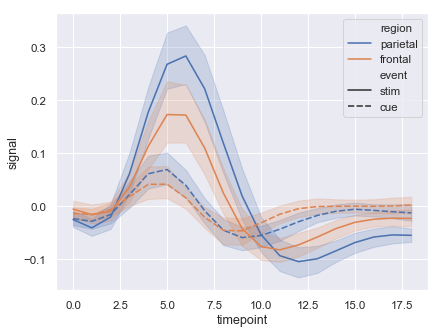
\includegraphics[width=\textwidth]{images/errorband_lineplots.png}
    \subcaption{Subfigure 1.}
    \label{fig:subcaption-subfigure1}
\end{subfigure}
\begin{subfigure}[b]{0.32\linewidth}
    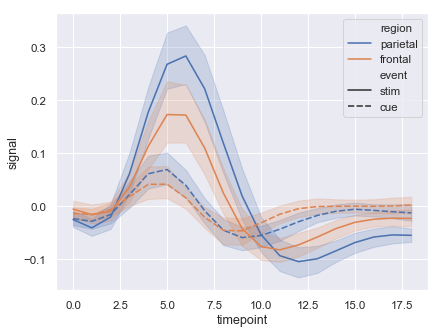
\includegraphics[width=\textwidth]{images/errorband_lineplots.png}
    \subcaption{Subfigure 2.}
    \label{fig:subcaption-subfigure2}
\end{subfigure}
\begin{subfigure}[b]{0.32\linewidth}
    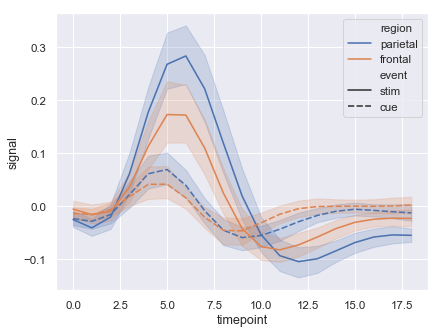
\includegraphics[width=\textwidth]{images/errorband_lineplots.png}
    \subcaption{Subfigure 3.}
    \label{fig:subcaption-subfigure3}
\end{subfigure}
\caption{Some sub-figures using \texttt{subcaption}.}
\label{fig:subcaption-subfigures}
\end{figure}
